\documentclass{article}
\usepackage{tikz}

\begin{document}

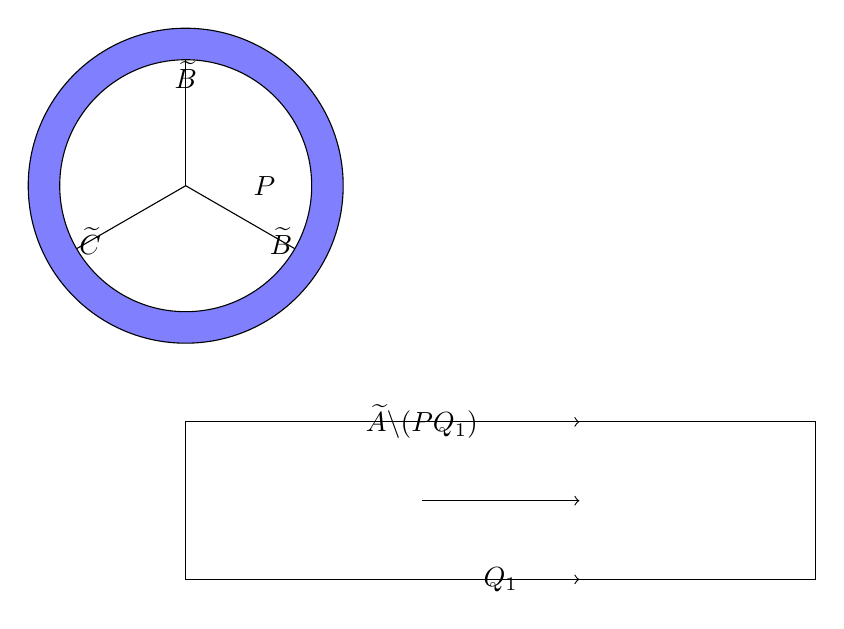
\begin{tikzpicture}[scale=2]
    % Draw the outer circle
    \draw[fill=blue!50] (0,0) circle (1);
    
    % Draw the inner circle
    \draw[fill=white] (0,0) circle (0.8);
    
    % Label the sections
    \node at (90:0.7) {$\widetilde{B}$};
    \node at (-30:0.7) {$\widetilde{B}$};
    \node at (210:0.7) {$\widetilde{C}$};
    
    % Draw the lines connecting the sections
    \draw (0,0) -- (90:0.8);
    \draw (0,0) -- (-30:0.8);
    \draw (0,0) -- (210:0.8);
    
    % Draw the rectangle and labels
    \draw (0,-1.5) rectangle (4,-2.5);
    \node at (2,-2.5) {$Q_{1}$};
    \node at (1.5,-1.5) {$\widetilde{A}\backslash(PQ_{1})$};
    
    % Draw the arrows
    \draw[->] (1.5,-1.5) -- (2.5,-1.5);
    \draw[->] (1.5,-2) -- (2.5,-2);
    \draw[->] (1.5,-2.5) -- (2.5,-2.5);
    
    % Label the point P
    \node at (0.5,0) {$P$};
\end{tikzpicture}

\end{document}